% ML1 technical deep dive -- compile with:  latexmk -xelatex deep_dive.tex
\documentclass[11pt,a4paper]{article}

\usepackage[margin=2.3cm,top=2.4cm,bottom=2.4cm,headsep=0.8cm]{geometry}
\usepackage{amsmath}
\usepackage{fontspec}
\usepackage{unicode-math}
\setmainfont{Cambria}
\setsansfont{Segoe UI}
\setmonofont{Consolas}[Scale=0.88]
\setmathfont{Cambria Math}
\usepackage[english]{babel}
\usepackage{microtype}
\usepackage[table]{xcolor}
\usepackage{graphicx}
\usepackage{booktabs,tabularx,array}
\usepackage{enumitem}
\usepackage{tikz}
\usetikzlibrary{positioning,arrows.meta,calc,fit,backgrounds,shapes.geometric}
\usepackage{pgfplots}
\pgfplotsset{compat=1.18}
\usepackage[most]{tcolorbox}
\usepackage{fvextra}
\usepackage{titlesec}
\usepackage{fancyhdr}
\usepackage[hidelinks]{hyperref}

% ------------------------------------------------------------------ colors
\definecolor{ink}{HTML}{1A1A19}
\definecolor{ink2}{HTML}{52514E}
\definecolor{muted}{HTML}{85847F}
\definecolor{s1}{HTML}{2A78D6}
\definecolor{s2}{HTML}{EB6834}
\definecolor{s3}{HTML}{1BAF7A}
\definecolor{s7}{HTML}{6250D6}
\definecolor{good}{HTML}{0CA30C}
\definecolor{warning}{HTML}{FAB219}
\definecolor{serious}{HTML}{EC835A}
\definecolor{critical}{HTML}{D03B3B}
\definecolor{track}{HTML}{F3F2EE}
\definecolor{gridc}{HTML}{E2E1DC}
\color{ink}

% ------------------------------------------------------------------ layout
\setlength{\parindent}{0pt}
\setlength{\parskip}{0.55em}
\linespread{1.08}
\setlist{itemsep=0.25em,topsep=0.3em}
\titleformat{\section}{\sffamily\Large\bfseries}{\color{s1}\thesection}{0.7em}{}
\titleformat{\subsection}{\sffamily\large\bfseries}{\color{s1}\thesubsection}{0.6em}{}
\titleformat{\subsubsection}{\sffamily\normalsize\bfseries}{}{0em}{}
\titlespacing*{\section}{0pt}{1.4em}{0.6em}
\titlespacing*{\subsection}{0pt}{1.1em}{0.4em}
\pagestyle{fancy}
\fancyhf{}
\fancyhead[L]{\sffamily\footnotesize\color{muted}Vigil · ML1 technical deep dive}
\fancyhead[R]{\sffamily\footnotesize\color{muted}\leftmark}
\fancyfoot[C]{\sffamily\footnotesize\color{muted}\thepage}
\renewcommand{\headrulewidth}{0.4pt}
\renewcommand{\headrule}{\color{gridc}\hrule height\headrulewidth}
\renewcommand{\sectionmark}[1]{\markboth{#1}{}}
\renewcommand{\arraystretch}{1.25}

% ------------------------------------------------------------------ helpers
\newcommand{\code}[1]{\texttt{\detokenize{#1}}}
\newcommand{\fref}[2]{\texttt{\textcolor{s1}{\detokenize{#1}:#2}}}
\newcommand{\fname}[1]{\texttt{\textcolor{s1}{\detokenize{#1}}}}
\newcommand{\badge}[2]{\tikz[baseline=(b.base)]\node[fill=#1,rounded corners=2pt,inner sep=2.2pt,font=\sffamily\bfseries\footnotesize,text=black](b){#2};}
\newcommand{\sevzero}{\badge{good}{0}}
\newcommand{\sevone}{\badge{warning}{1}}
\newcommand{\sevtwo}{\badge{serious}{2}}
\newcommand{\sevthree}{\badge{critical}{\textcolor{white}{3}}}
\newcolumntype{Y}{>{\raggedright\arraybackslash}X}
\newcommand{\thead}[1]{\sffamily\bfseries\small #1}

\tcbset{boxbase/.style={enhanced,breakable,boxrule=0pt,leftrule=3pt,arc=1.5pt,
  left=8pt,right=8pt,top=6pt,bottom=6pt,fonttitle=\sffamily\bfseries\small,
  before skip=0.8em,after skip=0.8em}}
\newtcolorbox{keyidea}[1][Key idea]{boxbase,colback=s1!6,colframe=s1,coltitle=s1!85!black,colbacktitle=s1!6,title={#1},
  attach title to upper,after title={\par\smallskip}}
\newtcolorbox{measured}[1][Measured]{boxbase,colback=good!7,colframe=good,coltitle=good!70!black,colbacktitle=good!7,title={#1},
  attach title to upper,after title={\par\smallskip}}
\newtcolorbox{pitfall}[1][Pitfall found by measuring]{boxbase,colback=critical!6,colframe=critical,coltitle=critical!85!black,colbacktitle=critical!6,title={#1},
  attach title to upper,after title={\par\smallskip}}
\newtcolorbox{trybox}[1][Try it]{boxbase,before upper=\raggedright,colback=s7!6,colframe=s7,coltitle=s7!85!black,colbacktitle=s7!6,title={#1},
  attach title to upper,after title={\par\smallskip}}

\tcbset{codebox/.style={enhanced,breakable,colback=track,colframe=track,boxrule=0pt,arc=1.5pt,
  left=6pt,right=6pt,top=3pt,bottom=3pt,before skip=0.6em,after skip=0.6em}}
\newenvironment{codeblock}{\VerbatimEnvironment\begin{tcolorbox}[codebox]%
  \begin{Verbatim}[breaklines,breakanywhere,fontsize=\small]}{\end{Verbatim}\end{tcolorbox}}

\tikzset{
  box/.style={draw=#1,fill=#1!8,rounded corners=3pt,thick,align=center,font=\sffamily\small,inner sep=5pt,minimum height=0.9cm},
  box/.default=s1,
  arr/.style={-{Stealth[length=2.4mm]},thick,color=ink2},
  lbl/.style={font=\sffamily\scriptsize,color=ink2}
}

\hypersetup{pdftitle={ML1 technical deep dive},pdfauthor={Vigil ML1}}

% ======================================================================
\begin{document}

% ------------------------------------------------------------- title page
\begin{titlepage}
\thispagestyle{empty}
\vspace*{1.2cm}
{\sffamily\color{s1}\bfseries\large VIGIL · DRIVER MONITORING\par}
\vspace{0.4cm}
{\sffamily\bfseries\fontsize{30}{36}\selectfont ML1 decision engine\par}
\vspace{0.2cm}
{\sffamily\fontsize{18}{24}\selectfont\color{ink2} A technical deep dive\par}
\vspace{1.0cm}
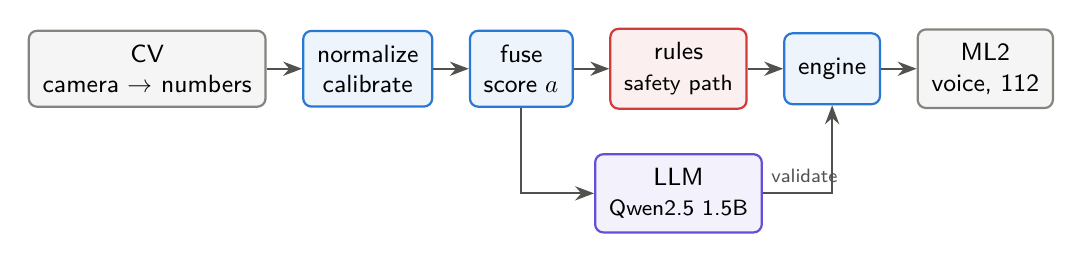
\begin{tikzpicture}[node distance=0.45cm and 0.45cm]
  \node[box=muted] (cv) {CV\\ camera $\to$ numbers};
  \node[box,right=of cv] (n) {normalize\\ calibrate};
  \node[box,right=of n] (f) {fuse\\ score $a$};
  \node[box=critical,right=of f] (r) {rules\\ \footnotesize safety path};
  \node[box=s7,below=0.55cm of r] (l) {LLM\\ \footnotesize Qwen2.5 1.5B};
  \node[box,right=of r] (e) {engine};
  \node[box=muted,right=of e] (m) {ML2\\ voice, 112};
  \draw[arr] (cv)--(n); \draw[arr] (n)--(f); \draw[arr] (f)--(r); \draw[arr] (r)--(e); \draw[arr] (e)--(m);
  \draw[arr] (f) |- (l); \draw[arr] (l) -| node[lbl,pos=0.3,above]{validate} (e);
\end{tikzpicture}
\vspace{1.2cm}

\begin{minipage}{0.92\textwidth}\large
How a camera frame becomes a decision: the math of the attention score, the rule ladder, how a
1.5B-parameter model is fenced in, the engine's state machine, and how all of it was measured.
\end{minipage}

\begin{keyidea}[How to read this]
\begin{tabularx}{\linewidth}{@{}l Y@{}}
\textbf{30 minutes} & Section 1 (mental model) $\to$ Section 2 (one frame's journey) $\to$ Section 6 (limitations) \\
\textbf{2 hours} & add 3.3 fusion, 3.4 rules, 3.7 validation, 3.8 engine, and exercises 1--4 \\
\textbf{a day} & everything in order, with the code open next to it, and all exercises \\
\end{tabularx}
\end{keyidea}

\vfill
\begin{tabularx}{\textwidth}{@{}l Y@{}}
\toprule
\thead{For} & the ML1 owner and anyone who must explain, debug or extend the decision engine \\
\thead{Assumes} & Python and the ML course basics (lectures C1--C6) \\
\thead{Measured on} & demo laptop, NVIDIA RTX 4050 6\,GB, Ollama, \code{qwen2.5:1.5b} (Q4\_K\_M) \\
\thead{Code} & every reference like \fref{fusion.py}{209} points to \code{ml1/<file>:<line>} in the repository \\
\thead{Companions} & \fname{docs/ARCHITECTURE.md}, \fname{docs/ML_METHODS.md}, \fname{docs/EVALUATION.md} \\
\bottomrule
\end{tabularx}
\end{titlepage}

\tableofcontents
\newpage

% ======================================================================
\section{The mental model}

\begin{center}
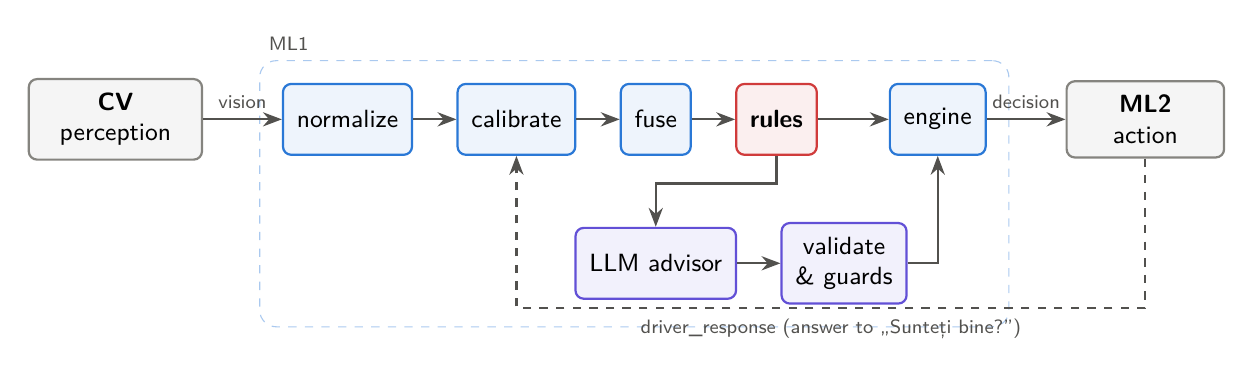
\begin{tikzpicture}[node distance=0.5cm and 0.55cm]
  \node[box=muted,minimum width=2.2cm] (cv) {\textbf{CV}\\ perception};
  \node[box,right=1.0cm of cv] (n) {normalize};
  \node[box,right=of n] (c) {calibrate};
  \node[box,right=of c] (f) {fuse};
  \node[box=critical,right=of f] (r) {\textbf{rules}};
  \node[box=s7,below=0.9cm of f] (l) {LLM advisor};
  \node[box=s7,right=of l] (v) {validate\\ \& guards};
  \node[box,right=0.9cm of r] (e) {engine};
  \node[box=muted,right=1.0cm of e,minimum width=2.0cm] (m) {\textbf{ML2}\\ action};
  \draw[arr] (cv)--node[lbl,above]{vision}(n);
  \draw[arr] (n)--(c); \draw[arr] (c)--(f); \draw[arr] (f)--(r); \draw[arr] (r)--(e);
  \draw[arr] (e)--node[lbl,above]{decision}(m);
  \draw[arr] (r.south) |- ++(0,-0.35) -| (l.north);
  \draw[arr] (l)--(v); \draw[arr] (v.east) -| (e.south);
  \draw[arr,dashed] (m.south) |- ++(0,-1.9) -| node[lbl,pos=0.25,below]{driver\_response (answer to „Sunteți bine?”)} (c.south);
  \begin{scope}[on background layer]
    \node[draw=s1!40,dashed,rounded corners=6pt,fit=(n)(r)(l)(v)(e),inner sep=8pt,label={[lbl,anchor=south west]north west:ML1}] {};
  \end{scope}
\end{tikzpicture}
\end{center}

Three ideas carry the whole design. Remember these and you can reconstruct the rest.

\begin{keyidea}[1 · Deterministic core, probabilistic advisor]
The rules (\fname{rules.py}) decide what is safety-relevant. The LLM refines inside limits the rules
set. This is the ISO 26262 pattern: the part that can cause harm, a false 112 call or a missed
emergency, must be testable and explainable.
\end{keyidea}

\begin{keyidea}[2 · Time is a signal]
Almost every hard case is about duration: a 1\,s glance vs 6\,s on the phone, a 1.5\,s chest touch vs
5\,s with heavy breathing, one lost face frame vs 1\,s of absence. Smoothing, persistence thresholds,
hysteresis and timeouts are where most of the logic lives.
\end{keyidea}

\begin{keyidea}[3 · Measure, don't assume]
Several ``obvious'' choices were wrong until measured: the prompt size, the LLM's value, the calibration
effect, a 0.1\,s latency. The red boxes in this document show each one.
\end{keyidea}

\subsection{Invariants: what must always stay true}

\begin{tabularx}{\textwidth}{@{}Y l@{}}
\toprule
\thead{Invariant} & \thead{Enforced in} \\
\midrule
A clear severity-3 case is never downgraded by the LLM & \fref{validate.py}{255} \\
The LLM never raises severity above the rules (\code{LLM_MAX_RAISE = 0}) & \fref{validate.py}{263} \\
112 only at severity 3 \emph{and} no answer or distress to „Sunteți bine?” & \fref{rules.py}{127}, \fref{validate.py}{307} \\
112 at most once per episode; no question repeated while waiting & \fref{engine.py}{223} \\
Severity 3 never waits for the LLM (fast path) & \fref{engine.py}{118} \\
The driver only hears pre-written Romanian phrases & \fref{actions.py}{17} \\
Any LLM failure (timeout, crash, invalid JSON) still yields a valid rule decision & \fref{validate.py}{341} \\
\bottomrule
\end{tabularx}

% ======================================================================
\section{One frame's journey (a real trace)}

The input is a frame from the CV team's own fake generator (\fname{Vision/vigil_vision/fake}), phase
\code{chest}, at $t = 45.0$\,s, after the earlier phases of their demo. Every number below was printed by
the code; exercise 1 reproduces it.

\subsection{Raw CV message}
\begin{codeblock}
{"ear": 0.29, "perclos": 0.05, "blink_rate": 34.0, "gaze_on_road": true,
 "head_drop": false, "phone": 0.0,
 "breathing": {"state": "heavy", "rate_bpm": 32.0, "amp_ratio": 3.1, "mouth_open": true},
 "posture":   {"state": "upright", "still_sec": 0.0},
 "events": [{"event": "hand_on_chest",   "duration_sec": 5.0, "confidence": 0.8, "breathing": "heavy"},
            {"event": "heavy_breathing", "duration_sec": 4.0, "confidence": 0.75}],
 "ts": 45.0, "camera_on": true, "face_detected": true, "landmarks": ["... 468 points ..."]}
\end{codeblock}

\subsection[Normalize]{Normalize \hfill\normalfont\small\fref{cv_adapter.py}{44}}
Landmarks are dropped, \code{breathing.state} becomes \code{breathing_state: "heavy"},
\code{posture.state} becomes \code{posture_state: "upright"}, and numbers are clipped to physical ranges.
Event names would be mapped here too (\code{phone_use} $\to$ \code{phone_in_hand}); this frame needs none.

\subsection[Fuse]{Fuse \hfill\normalfont\small\fref{fusion.py}{209}}
Each available signal gets a sub-score $s_i\in[0,1]$, where 1 means attentive.

\begin{tabularx}{\textwidth}{@{}l c c Y@{}}
\toprule
\thead{Signal} & \thead{Weight} & \thead{$s_i$} & \thead{Why} \\
\midrule
eyes   & 0.30 & 1.000 & PERCLOS 0.05; EAR 0.29 $\approx$ the driver's calibrated 0.30 \\
gaze   & 0.15 & 1.000 & on road \\
head   & 0.15 & 1.000 & not dropped \\
phone  & 0.15 & 1.000 & score 0.0 \\
blink  & 0.05 & 0.686 & 34/min vs personal normal 15.4: upper limit $\max(25, 1.8\cdot15.4)=27.7$, ramp to 47.7, so $(47.7-34)/20$ \\
events & 0.10 & 0.280 & hand on chest + heavy breathing: penalty $\max(0.6\cdot0.8,\;0.9\cdot0.8)\cdot1.0 = 0.72$ \\
\bottomrule
\end{tabularx}

Only available signals count (voice and driving are absent), so the weights are re-normalized over
their sum, 0.90:
\[
\text{weighted} \;=\; \frac{\sum_i w_i s_i}{\sum_i w_i}
 \;=\; 0.333 + 0.167 + 0.167 + 0.167 + 0.056\cdot0.686 + 0.111\cdot0.28 \;=\; 0.903 .
\]

A score of 0.903 would describe an attentive driver. That is why \textbf{caps} exist
(\fref{fusion.py}{61}): a serious signal limits the total instead of being averaged away.
\[
\text{cap}_i = f_i + (1-f_i)\,s_i ,\qquad
\text{cap}_\text{events} = 0.40 + 0.60\cdot0.28 = 0.568 ,\qquad
a_\text{raw} = \min(0.903,\;0.568) = 0.568 .
\]

\begin{center}
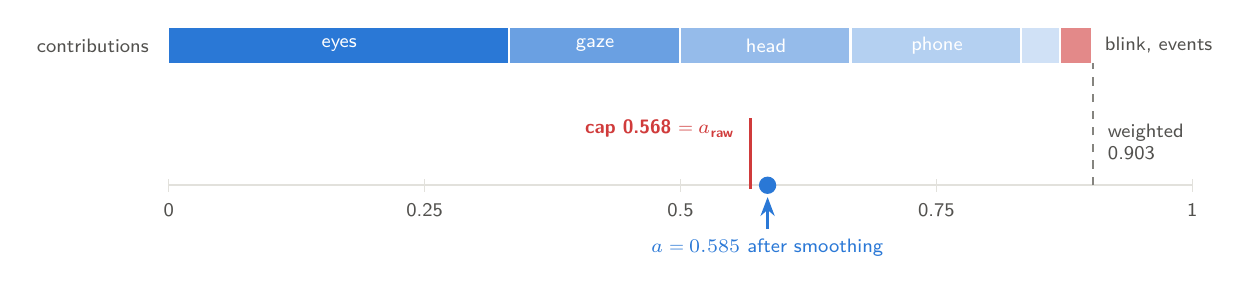
\begin{tikzpicture}[x=13cm,y=1cm]
  % stacked contributions
  \def\y{1.55}
  \foreach \a/\b/\c/\t in {0/0.333/s1/eyes,0.333/0.5/s1!70/gaze,0.5/0.667/s1!50/head,0.667/0.834/s1!35/phone,0.834/0.872/s1!22/,0.872/0.903/critical!60/}{
    \fill[\c] (\a,\y) rectangle ($(\b,\y+0.45)-(0.002,0)$);
    \node[font=\sffamily\scriptsize,text=white] at ({(\a+\b)/2},\y+0.225) {\t};
  }
  \node[lbl,anchor=west] at (0.905,\y+0.225) {blink, events};
  \node[lbl,anchor=east] at (-0.01,\y+0.225) {contributions};
  % axis
  \draw[gridc,thick] (0,0)--(1,0);
  \foreach \v in {0,0.25,0.5,0.75,1} {\draw[gridc] (\v,-0.08)--(\v,0.08); \node[lbl,below] at (\v,-0.1) {\v};}
  \draw[muted,thick,dashed] (0.903,0)--(0.903,\y);
  \node[lbl,anchor=west,align=left] at (0.908,0.55) {weighted\\0.903};
  \draw[critical,very thick] (0.568,-0.05)--(0.568,0.85);
  \node[anchor=east,font=\sffamily\scriptsize\bfseries,text=critical] at (0.562,0.72) {cap 0.568 $= a_\text{raw}$};
  \fill[s1] (0.585,0) circle (0.11cm);
  \draw[arr,s1] (0.585,-0.55) node[below,font=\sffamily\scriptsize,text=s1]{$a=0.585$ after smoothing}--(0.585,-0.15);
\end{tikzpicture}
\end{center}

Then comes \textbf{asymmetric smoothing} (\fref{fusion.py}{280}), an exponential moving average whose
time constant depends on the direction:
\[
\alpha = 1 - e^{-\Delta t/\tau},\qquad a \leftarrow a + \alpha\,(a_\text{raw}-a),\qquad
\tau=\begin{cases}0.7\text{ s} & a_\text{raw} < a \ \text{(falling)}\\ 4.0\text{ s} & a_\text{raw} > a \ \text{(rising)}\end{cases}
\]

\begin{center}
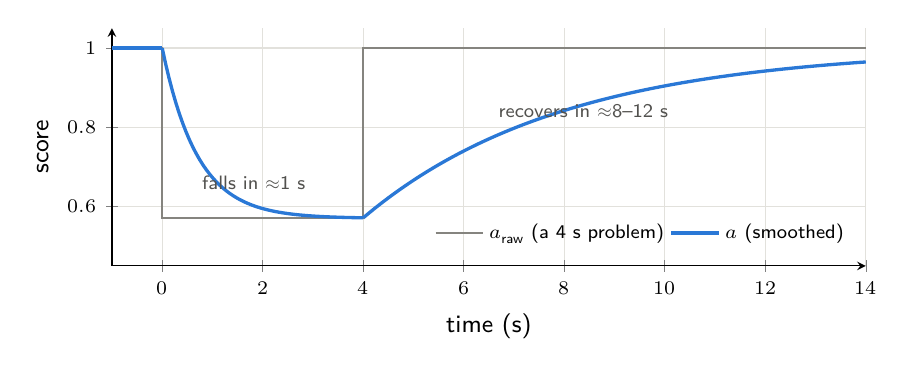
\begin{tikzpicture}
\begin{axis}[width=0.92\textwidth,height=4.6cm,xmin=-1,xmax=14,ymin=0.45,ymax=1.05,
  axis lines=left,xlabel={time (s)},ylabel={score},label style={font=\sffamily\small},
  tick label style={font=\sffamily\scriptsize},grid=major,grid style={gridc},
  legend style={font=\sffamily\scriptsize,draw=none,fill=none,at={(0.99,0.05)},anchor=south east},legend columns=2]
  \addplot[muted,thick,const plot] coordinates {(-1,1) (0,1) (0,0.57) (4,0.57) (4,1) (14,1)};
  \addlegendentry{$a_\text{raw}$ (a 4 s problem)}
  \addplot[s1,very thick,domain=0:4,samples=60] {0.57+0.43*exp(-x/0.7)};
  \addlegendentry{$a$ (smoothed)}
  \addplot[s1,very thick,domain=4:14,samples=80,forget plot] {1-(1-(0.57+0.43*exp(-4/0.7)))*exp(-(x-4)/4)};
  \addplot[s1,very thick,forget plot] coordinates {(-1,1) (0,1)};
  \node[font=\sffamily\scriptsize,text=ink2,anchor=west] at (axis cs:0.6,0.66) {falls in $\approx$1 s};
  \node[font=\sffamily\scriptsize,text=ink2,anchor=west] at (axis cs:6.5,0.84) {recovers in $\approx$8--12 s};
\end{axis}
\end{tikzpicture}
\end{center}

Result: $a = 0.585$, slightly behind $a_\text{raw}$. Falling fast means a real problem shows within about
a second; rising slowly means one good frame cannot ``un-alarm'' the system. \textbf{Confidence} is 0.60:
camera only. The voice and driving sources each add 0.2 when present.

\subsection[Calibrate]{Calibrate \hfill\normalfont\small\fref{calibration.py}{46}}
Calibration finished in the first 30\,s of this trip: \code{ear = 0.30}, \code{blink = 15.4},
\code{perclos_offset = 0.0}. That is where the blink sub-score's personal limits came from.

\subsection[Rules]{Rules \hfill\normalfont\small\fref{rules.py}{74}}
\begin{codeblock}
rule_severity  ->  (3, "mână pe piept + respirație grea")
\end{codeblock}
Hand on chest for at least 3\,s with confidence at least 0.6, plus heavy breathing. Three sources are
accepted for the breathing: the event's \code{breathing} attribute, a \code{heavy_breathing} event, or
\code{breathing_state}. The context also carries:
\begin{codeblock}
"driver_response": {"answered": false, "timeout": true, "question": "Sunteți bine?"}
\end{codeblock}
The engine asked „Sunteți bine?” at 35.6\,s. Nobody answers in the CV demo (ML2 is not connected), so
after 8\,s of silence the engine records ``no answer'' (\fref{engine.py}{182}).

\subsection[Prompt]{Prompt \hfill\normalfont\small\fref{prompt.py}{59}}
\begin{codeblock}
a=0.58 conf=0.60 cam=on | perclos=0.05 ear=0.29 blink=34 | gaze_on_road=yes head_drop=no
phone=0.00 | breathing=heavy posture=upright | events: hand_on_chest 5s heavy, heavy_breathing 4s
| a 10s ago=0.39 | answer: no answer | hint=3
\end{codeblock}
The messages are a fixed system prompt, 5 fixed examples, and this one line.

\begin{measured}[Measured: where the LLM's time goes]
976 prompt tokens (Ollama's \code{prompt_eval_count}), but the prompt phase took only \textbf{9--18\,ms}:
the fixed prefix is reused from the KV cache. The whole call took about \textbf{330\,ms}.
Generating the answer is the cost, which is why the answer format is kept short.
\end{measured}

\subsection[LLM answer]{LLM answer \hfill\normalfont\small\fref{llm_client.py}{48}}
\begin{codeblock}
{"severity": 3, "actions": ["alarm", "esp32", "ask_ok"], "reason": "cap închis, răsfoarea grea 5 s"}
\end{codeblock}
42 output tokens. Three things to notice:
\begin{itemize}
  \item the JSON is valid and the actions come from the menu, guaranteed by schema-constrained decoding (3.5);
  \item the Romanian \code{reason} is garbled, which is why the model never writes what the driver hears;
  \item it \textbf{forgot \code{call_112}}, although the line says \code{answer: no answer} and the rules say 112 is due.
\end{itemize}

\subsection[Validate and guard]{Validate and guard \hfill\normalfont\small\fref{validate.py}{341}}
\begin{enumerate}
  \item \code{parse_llm_output} extracts the JSON;
  \item \code{expand_actions} turns \code{"alarm"} into \texttt{\{"tool": "play\_alarm", "args": \{"level": 3\}\}}, with the level taken from the severity;
  \item \code{validate_decision} checks known tools, typed arguments and a severity in 0..3;
  \item \code{apply_safety}: the rules say 112 is due and the LLM omitted it, so the guard \textbf{adds \code{call_112}}
        with the template report, and logs the note \emph{call\_112 adăugat: severitate 3 și șoferul nu a răspuns}.
\end{enumerate}

\subsection[Engine]{Engine \hfill\normalfont\small\fref{engine.py}{93}}
In the real run the \textbf{fast path} had already published 112 at 43.6\,s, the moment the rules saw
``severity 3 + no answer'', without waiting for the LLM. When this LLM decision arrives, \code{_publish}
strips the repeated \code{call_112} (112 once per episode), and de-duplication drops the decision because
it adds nothing new for the driver.

% ======================================================================
\section{Module by module}

\subsection{\texttt{cv\_adapter.py}: the boundary}
\begin{itemize}
  \item \fref{cv_adapter.py}{44} \code{normalize_vision} is the single place where the CV schema meets ML1.
        If CV renames a field or an event, only \code{EVENT_ALIASES} (\fref{cv_adapter.py}{23}) changes.
  \item Cleaning (C2): non-finite values become \code{None}; values are clipped to \code{RANGES}
        (\fref{cv_adapter.py}{31}). Clipping instead of dropping: a clipped value still carries information,
        a dropped frame does not.
  \item \fref{cv_adapter.py}{99} \code{cv_demo_messages} imports the CV team's generator from \fname{Vision/},
        so ML1 is tested on exactly the shape the camera produces.
\end{itemize}

\subsection{\texttt{calibration.py}: per-driver normalization}
Thresholds tuned on an ``average'' driver misfire on a driver with naturally narrow eyes (EAR 0.22,
measured PERCLOS 0.15).

\begin{pitfall}[Found by the evaluation]
On the shifted domain (narrow eyes, more noise, face often lost), the rules engine without calibration
raised \textbf{21 false alarms per hour}. With calibration: \textbf{0}, and macro-F1 went from
0.60\,[0.50--0.75] to 0.91\,[0.84--0.96]. The confidence intervals don't overlap.
\end{pitfall}

How \fref{calibration.py}{66} \code{DriverBaseline.update} works:
\begin{itemize}
  \item \textbf{Fit on the past only.} It learns from the first 30\,s and applies to later frames, never the
        reverse: the train/transform discipline from C2, applied in time.
  \item \textbf{Only clean frames} (\fref{calibration.py}{56}): face visible, gaze on road, no events, no
        phone. Otherwise a glance or a yawn would be learned as ``normal''.
  \item \textbf{Robust statistics.} Median and IQR, not mean and standard deviation. One long blink
        (EAR 0.01) barely moves a median but drags a mean.
  \item \textbf{Plausibility bounds} (\fref{calibration.py}{21}): a baseline PERCLOS above 0.20 is rejected.
        A driver who is already drowsy at the start must not teach the system that drowsy is normal.
  \item \textbf{Fallback.} After $3\times30$\,s without enough clean frames, population values are used.
\end{itemize}

\subsection{\texttt{fusion.py}: from signals to one score}
The constants are the model, so it matters where each one comes from.

{\small
\begin{tabularx}{\textwidth}{@{}>{\raggedright\arraybackslash}p{3.4cm} >{\raggedright\arraybackslash}p{3.6cm} Y >{\raggedright\arraybackslash}p{2.9cm}@{}}
\toprule
\thead{Constant} & \thead{Value} & \thead{Meaning} & \thead{Origin} \\
\midrule
\code{WEIGHTS} & eyes 0.30, gaze/head/phone 0.15, \dots & relative trust in each signal & hand-chosen \\
\code{CAPS} & eyes 0.35, events 0.40 & floor $f_i$ of the cap line & hand-chosen \\
\code{TAU_DOWN}, \code{TAU_UP} & 0.7\,s / 4.0\,s & smoothing time constants & hand-chosen \\
\code{EVENT_SEVERITY} & head drop 1.0, eyes closed 0.8, \dots & penalty per event type & eyes closed lowered after CV demo \\
\code{FACE_MISSING_SEC} & 1.0\,s & lost face = not looking, after this & \textbf{chosen from data} \\
\code{LOW_A} + persistence & 0.75 for 4\,s & generic ``reduced attention'' rule & \textbf{chosen from data} \\
\code{SOURCE_CONFIDENCE} & camera 0.6, voice 0.2, driving 0.2 & coverage-based confidence & hand-chosen, \emph{not calibrated} \\
\bottomrule
\end{tabularx}}

Two subtleties:
\begin{itemize}
  \item \textbf{\code{critical}} (\fref{fusion.py}{274}) bypasses smoothing: head dropped with eyes closed, a
        near-certain severe event, or no answer with eyes closed. Waiting a second for the moving average is
        unacceptable there.
  \item \textbf{Missing data is not neutral.} Camera off (privacy, the user's choice) means lower confidence,
        \emph{not} inattention. Face missing while the camera works means, after 1\,s, gaze = 0. The same
        ``missing value'' has a different mechanism (C2: MCAR vs MNAR) and therefore a different meaning.
\end{itemize}

\subsection{\texttt{rules.py}: the decision ladder}
\fref{rules.py}{74} \code{rule_severity} is an ordered ladder: \textbf{the first match wins}, from most to least
severe. The order is part of the meaning. Moving the ``eyes closed $\ge$ 1.5\,s $\to$ 2'' rung above
``eyes closed + no answer $\to$ 3'' would silently remove an emergency path.

\begin{tabularx}{\textwidth}{@{}c Y@{}}
\toprule
\thead{Sev.} & \thead{Condition (checked top to bottom)} \\
\midrule
\sevthree & fusion \code{critical} $\vee$ head drop with eyes closed $\vee$ \code{head_on_wheel} $\ge 2$\,s $\vee$ slumped and still $\ge 2$\,s \\
\sevthree & eyes closed $\ge 3$\,s, \emph{continuous in the EAR too} (not a tracker-merged episode) \\
\sevthree & eyes closed $\ge 1.5$\,s $\wedge$ (no answer $\vee$ distress) \\
\sevthree & hand on chest $\ge 3$\,s $\wedge$ heavy breathing \quad(\sevtwo\ if a quick, coherent „sunt bine”) \\
\sevthree & (no answer $\vee$ distress) $\wedge$ $a < 0.5$ \\
\sevtwo & eyes closed $\ge 1.5$\,s (microsleep) $\vee$ microsleep $\vee$ PERCLOS $\ge 0.15$ $\vee$ $a<0.5$ \\
\sevtwo & frequent yawning $\vee$ low blink rate $\ge 5$\,s with PERCLOS $\ge 0.12$ $\vee$ yawn with PERCLOS $\ge 0.12$ \\
\sevone & phone score $\ge 0.6$ $\vee$ phone event $\ge 2$\,s $\vee$ gaze off road $\ge 2$\,s $\vee$ \code{off_road_ratio} $\ge 0.5$ \\
\sevzero & short medical sign ($<3$\,s): watch, don't remind the driver to look at the road \\
\sevone & $a < 0.75$ for at least 4\,s \\
\sevzero & otherwise \\
\bottomrule
\end{tabularx}

Eye closures during a yawn or while looking down (phone) are \textbf{artifacts} and never count as
microsleep, including a closure episode that began during one (a rule taken from the CV team's
\fname{alerts.py}). ``PERCLOS'' is the 15\,s closure fraction when available (from CV, or ML1's own
estimate, used only if consistent with CV's 60\,s value), otherwise CV's 60\,s value corrected by
calibration. All these thresholds live in \fname{profile.py} (Section 3.9).

\fref{rules.py}{60} \code{answer_status} turns ML2's answer into \code{none / no_answer / distress / slow / ok}
with two regular expressions. It is crude (Section 6), but deterministic and testable.

\fref{rules.py}{127} \code{wants_112}: severity 3 and (no answer or distress) \textbf{to „Sunteți bine?”}.
Silence after „Doriți o pauză?” first escalates to an urgent check, never straight to 112.

\subsection{\texttt{actions.py} and \texttt{prompt.py}: constraining a small model}
A 1.5B model is unreliable at free-form generation and at native function calling, so its job is narrowed
to choosing a severity and picking items from a menu.

\begin{itemize}
  \item \textbf{Menu} (\fname{actions.py}): 8 action IDs; alarm levels derived from the severity; phrases fixed.
  \item \textbf{Schema-constrained decoding} (\fref{actions.py}{43}): the JSON schema is sent as Ollama's
        \code{format}. llama.cpp compiles it into a grammar and, while sampling, masks every token that would
        violate it. The model \emph{cannot} emit invalid JSON or an action outside the enum. It can still pick
        a wrong but valid action, as in 2.7, which is why validation exists.
  \item \textbf{Static prefix} (\fref{prompt.py}{19}): system prompt and examples are byte-identical on every
        call, so the server reuses their KV cache. Any per-call content in the prefix, such as a timestamp,
        would break this.
  \item \textbf{\code{hint=}}: the rule severity is given to the model. It anchors a small model; the model's
        job becomes ``agree, or argue down one level with context''.
\end{itemize}

\begin{pitfall}[Found while writing this document]
The prompt was assumed to be about 800 tokens; Ollama measured \textbf{976}. With up to 48 output tokens,
that overflowed the 1024-token context, and Ollama then drops the \emph{beginning} of the prompt, which is
where the rules are. Fix: \code{num_ctx = 2048} (memory still 1.1\,GB) and a token estimate recalibrated to
2.8 characters per token, which now predicts 975 against 976 measured.
\end{pitfall}

\subsection{\texttt{llm\_client.py}: inference settings}
\begin{tabularx}{\textwidth}{@{}l l Y@{}}
\toprule
\thead{Option} & \thead{Value} & \thead{Why} \\
\midrule
\code{temperature}, \code{top_k}, \code{seed} & 0, 1, 42 & deterministic, reproducible decisions \\
\code{num_predict} & 48 & an answer is 25--42 tokens; caps worst-case latency \\
\code{num_ctx} & 2048 & room for the 976-token prompt plus the answer \\
\code{keep_alive} & 60 min & no model reload between calls \\
\code{warmup()} & same options & loading takes $\approx$3\,s ($\approx$90\,s cold after a reboot); changing any option above \textbf{reloads the model} \\
\bottomrule
\end{tabularx}

\subsection{\texttt{validate.py}: the trust boundary}
\fref{validate.py}{341} \code{decide} never raises an exception.

\begin{center}
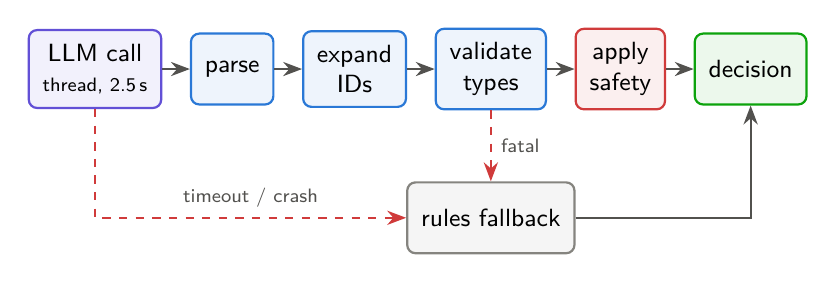
\begin{tikzpicture}[node distance=0.35cm]
  \node[box=s7] (l) {LLM call\\ \scriptsize thread, 2.5\,s};
  \node[box,right=of l] (p) {parse};
  \node[box,right=of p] (x) {expand\\ IDs};
  \node[box,right=of x] (v) {validate\\ types};
  \node[box=critical,right=of v] (s) {apply\\ safety};
  \node[box=good,right=of s] (o) {decision};
  \node[box=muted,below=0.9cm of v] (fb) {rules fallback};
  \foreach \a/\b in {l/p,p/x,x/v,v/s,s/o} \draw[arr] (\a)--(\b);
  \draw[arr,dashed,critical] (l.south) |- node[lbl,pos=0.75,above]{timeout / crash} (fb.west);
  \draw[arr,dashed,critical] (v.south)--node[lbl,right]{fatal} (fb.north);
  \draw[arr] (fb.east) -| (o.south);
\end{tikzpicture}
\end{center}

The guards in \code{apply_safety}, in order:
\begin{enumerate}[label=\textbf{\arabic*}]
  \item \textbf{floor}: severity $\ge$ (3 if rules = 3, else rules $-$ 1)
  \item \textbf{ceiling}: severity $\le$ rules + \code{LLM_MAX_RAISE} (= rules); 0 if rules = 0
  \item \textbf{evidence}: phone and road reminders need the matching sign in the data
  \item \textbf{voice}: severity $\ge 2$ gets a question; at 3 the question is „Sunteți bine?”
  \item \textbf{112}: removed without evidence, added when due
  \item \textbf{levels}: alarm and ESP32 level $\le$ severity; severity 3 forces level 3
  \item \textbf{empty}: severity $>0$ with no valid action gets the standard actions
\end{enumerate}
Every intervention is logged in \code{safety_notes} and shown on the dashboard. On the 5 benchmark
contexts the guards intervene on 20\% of answers (the drowsy case omits the voice question).

\subsection{\texttt{engine.py}: the state machine}

\begin{center}
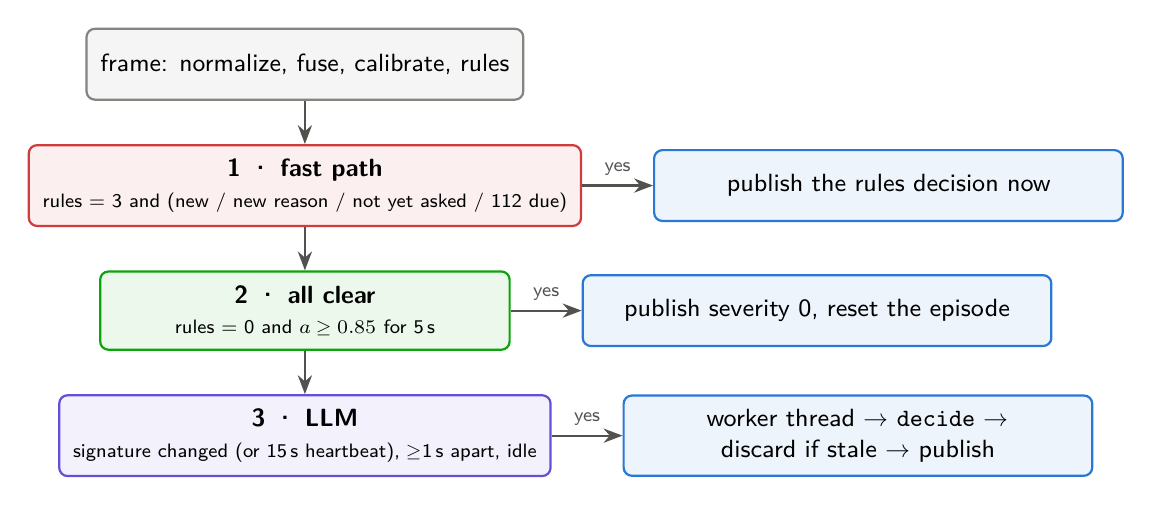
\begin{tikzpicture}[node distance=0.55cm and 0.9cm]
  \node[box=muted,minimum width=5.2cm] (in) {frame: normalize, fuse, calibrate, rules};
  \node[box=critical,below=of in,minimum width=5.2cm] (fp) {\textbf{1 · fast path}\\ \scriptsize rules = 3 and (new / new reason / not yet asked / 112 due)};
  \node[box=good,below=of fp,minimum width=5.2cm] (ac) {\textbf{2 · all clear}\\ \scriptsize rules = 0 and $a\ge0.85$ for 5\,s};
  \node[box=s7,below=of ac,minimum width=5.2cm] (ll) {\textbf{3 · LLM}\\ \scriptsize signature changed (or 15\,s heartbeat), $\ge$1\,s apart, idle};
  \node[box,right=of fp,text width=5.6cm] (fpa) {publish the rules decision now};
  \node[box,right=of ac,text width=5.6cm] (aca) {publish severity 0, reset the episode};
  \node[box,right=of ll,text width=5.6cm] (lla) {worker thread $\to$ \code{decide} $\to$ discard if stale $\to$ publish};
  \draw[arr] (in)--(fp); \draw[arr] (fp)--(ac); \draw[arr] (ac)--(ll);
  \draw[arr] (fp)--node[lbl,above]{yes}(fpa); \draw[arr] (ac)--node[lbl,above]{yes}(aca); \draw[arr] (ll)--node[lbl,above]{yes}(lla);
\end{tikzpicture}
\end{center}

The LLM \textbf{signature} is (rule severity, active events, $a$ in quarters, answer status). The LLM is
called only when the signature changes, which gives about 11 calls per 150 frames of drowsiness and 0
during calm driving.

\begin{tabularx}{\textwidth}{@{}l >{\raggedright\arraybackslash}p{4.4cm} Y@{}}
\toprule
\thead{Timer} & \thead{Value} & \thead{Effect} \\
\midrule
\code{ask_timeout} & 8\,s & silence after a question counts as ``no answer'' (works even if ML2 or speech recognition is down) \\
all clear & 5\,s of calm & prevents flicker between episodes \\
downgrade & 5\,s lower, never while awaiting an answer & stable severity \\
\code{min_gap} / \code{heartbeat} & 1\,s / 15\,s & LLM rate limit \\
\bottomrule
\end{tabularx}

\textbf{Async mode} (\code{sync=False}, used by the dashboard and the MQTT bridge): the LLM runs in a worker
thread. When its answer returns, \fref{engine.py}{200} \code{_llm_job} discards it if a newer decision was
published meanwhile, or if it would fall below the \emph{current} rule floor. A slow LLM can never overwrite a
newer fast-path decision.

\textbf{Publishing} (\fref{engine.py}{223}): strips a repeated \code{call_112}, strips questions after 112 or
while awaiting an answer, and, for LLM decisions, drops anything that adds nothing new for the driver.

\subsection{\texttt{profile.py}: thresholds that depend on how CV measures}
Reading the CV team's code (\fname{Vision/vigil_vision/face/eyes.py}, \fname{alerts.py}, \fname{events/tracker.py})
changed several assumptions. The thresholds that depend on CV's definitions are now one profile, and the
evaluation compares profiles on validation data.

\begin{tabularx}{\textwidth}{@{}>{\raggedright\arraybackslash}p{3.3cm} Y Y@{}}
\toprule
\thead{Signal} & \thead{How CV measures it} & \thead{What ML1 does now} \\
\midrule
PERCLOS & fraction of time with eyes \emph{almost fully} closed over \textbf{60\,s}; normal $\le0.05$; null for 10\,s & fatigue at $\ge 0.15$ (CV's own threshold, was 0.35); 15\,s estimate for fast onset and recovery \\
\code{eyes_closed} event & tracker merges activations separated by $<1$\,s: duration = episode & 1.5\,s $\to$ 2; 3\,s $\to$ 3 only if continuous in the EAR \\
yawn / looking down & eyelids look closed; CV's alerts exclude them & excluded as artifacts \\
\code{head_drop} & face \emph{or} slumped body (no face needed) & collapse without requiring PERCLOS \\
first 30\,s & CV calibrates its own thresholds & ML1 uses a provisional baseline (running median) \\
\bottomrule
\end{tabularx}

\begin{pitfall}[Found by rewriting the simulator in CV's real semantics]
On the realistic simulator the \emph{old} thresholds and even the first CV-aligned version scored poorly
(validation macro-F1 0.49--0.67): the 60\,s PERCLOS lag kept fatigue alarms on for up to a minute after recovery,
merged blink episodes looked like 3\,s eye closures, and narrow-eyed drivers were judged against the population
during calibration. After the fixes: validation cost 0.17 $\to$ 0.12, test macro-F1 0.75 $\to$ 0.83.
\end{pitfall}

\subsection{\texttt{service.py} and \texttt{http\_api.py}: the live path}
The future input is a Spring Boot server fed by a live camera. One transport-independent service handles what
a live stream brings: missing timestamps (server clock), milliseconds or ISO-8601 (Java), camelCase field names
(Jackson), envelopes like \texttt{\{"type", "payload"\}}, duplicates, frames more than 0.5\,s late, gaps over 30\,s,
and a driver change (\code{/reset}). HTTP adds REST for frames and Server-Sent Events for decisions (consumed
natively by Spring WebClient); MQTT uses the same service. The contract and Java examples are in
\fname{docs/API.md}.

\subsection{The rest}
\begin{itemize}
  \item \fname{reports.py}: 112 and post-trip reports from templates. Facts only; the ``suspicion'' line says
        ``signs observed by the camera, not a diagnosis''.
  \item \fname{mqtt_bridge.py}: \code{Bridge} holds all the logic and is tested without a broker; \code{run_mqtt}
        only wires it to paho. Not yet run against a real broker.
  \item \fname{dashboard.py} with \fname{web/index.html}: replays a scenario in real time through the same engine;
        the body comes from \fname{mock_pose.py}.
\end{itemize}

\begin{center}
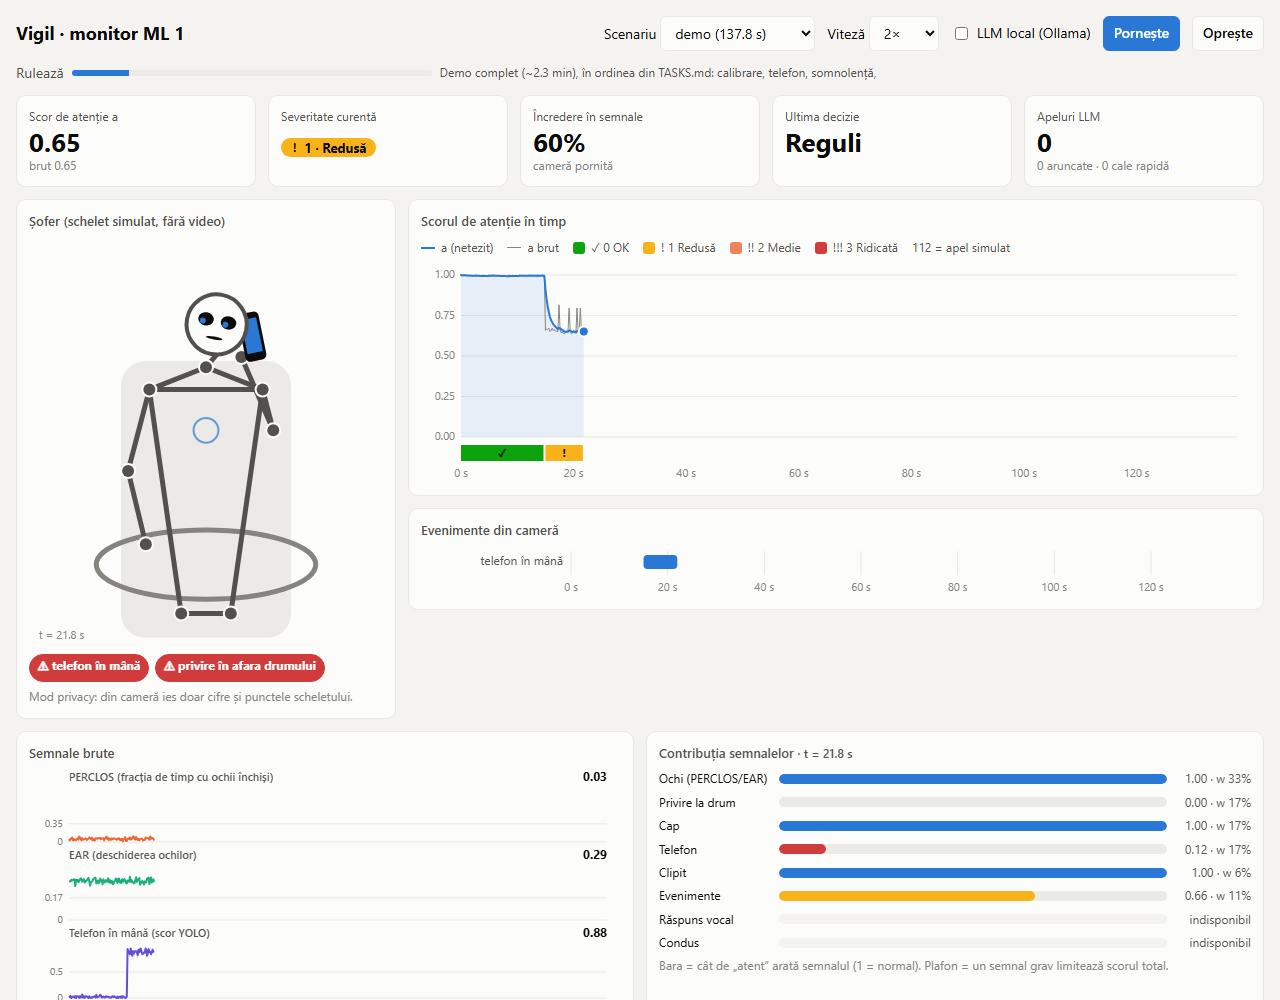
\includegraphics[width=0.95\textwidth]{../figures/dashboard_phone.png}\\[2pt]
{\small\color{ink2} The dashboard during the phone phase of the demo: the skeleton raises the phone, the score drops to 0.65 (severity 1).}
\end{center}

% ======================================================================
\section{Evaluation internals}

\begin{itemize}
  \item \textbf{Simulator} (\fref{evaluate.py}{122} \code{TripSim}): a latent state per frame (fatigue level $D$,
        phone, chest, collapse, \dots) becomes a CV-format message with driver-specific noise. Events are
        emitted only after CV's minimum durations.
  \item \textbf{Closed loop} (\fref{evaluate.py}{252} \code{respond}): answers depend on the true state and are
        drawn from a generator seeded per (trip, episode, question type), so compared variants receive identical answers.
  \item \textbf{Labels and grace windows} (\fref{evaluate.py}{235}): frames in the first 4\,s after a true
        escalation and 12\,s after a de-escalation are excluded (designed latency and hysteresis). Latency is
        measured separately.
  \item \textbf{Split by driver}: train 20 / validation 8 / test 10 / shift 8. Adjacent frames of one driver are
        nearly identical, so a split by frames would leak information (C5).
\end{itemize}

\begin{pitfall}[Two bugs in the evaluation itself]
\textbf{Unpaired randomness:} the simulated answers came from a shared random stream, so two variants asking at
slightly different moments got different answers, and calibration looked harmful by pure luck.
\textbf{Timestamp drift:} segment lengths weren't multiples of the 0.2\,s frame step, so timestamps drifted
from \code{index/5} by up to about 2\,s, producing impossible 0.1\,s latencies and an LLM ``gain'' that
disappeared once fixed.
\end{pitfall}

\subsection{Metrics}
From the $4\times4$ confusion matrix $C$ (rows = truth, columns = prediction):
\[
P_k = \frac{C_{kk}}{\sum_j C_{jk}},\qquad R_k = \frac{C_{kk}}{\sum_j C_{kj}},\qquad
F1_k = \frac{2P_kR_k}{P_k+R_k},\qquad \text{macro-F1} = \frac{1}{|K|}\sum_{k\in K} F1_k .
\]
Cost per frame is $\sum_{t,p} C_{tp}\,\text{COST}_{tp} / \sum C$ (\fref{evaluate.py}{49}), with
\[
\text{COST}_{tp} = \begin{cases} 5\,(t-p)\cdot(2 \text{ if } t=3 \text{ else } 1) & p<t \ \text{(under-estimate)}\\ p-t & p>t \ \text{(over-estimate)}\end{cases}
\]
So missing an emergency by one level costs $10\times$ as much as an over-alarm by one level.
\textbf{Bootstrap} (\fref{evaluate.py}{450}): resample \emph{trips}, not frames, with replacement 400 times,
recompute the metric from the summed confusion matrices, and report the 2.5--97.5 percentiles.

\subsection{Results}
\begin{tabularx}{\textwidth}{@{}Y c c c c@{}}
\toprule
\thead{Variant (test, unseen drivers)} & \thead{macro-F1 [95\% CI]} & \thead{cost} & \thead{false alarms/h} & \thead{112 correct} \\
\midrule
majority class (always 0) & 0.238 & 1.563 & -- & -- \\
threshold on $a$ (chosen on validation) & 0.388 & 0.135 & -- & -- \\
softmax regression (C4) & 0.953 & 0.041 & -- & -- \\
decision tree (C6) & 0.916 & 0.074 & -- & -- \\
rules, old thresholds (legacy) & 0.753 [0.64--0.85] & 0.171 & 18.2 & 6/6 \\
rules + calibration (CV-aligned) & 0.825 [0.76--0.87] & 0.090 & 13.6 & 6/6 \\
\textbf{LLM + rules + calibration} & \textbf{0.887 [0.82--0.94]} & \textbf{0.078} & 17.0 & 6/6 \\
\bottomrule
\end{tabularx}

\begin{keyidea}[How to read the near-perfect softmax and tree]
They learned the simulator that also produced the labels. That is an upper bound for ``what a learned model
could do with labels'', not a real-world estimate. The LLM's gain over the rules (0.887 vs 0.825) has
overlapping intervals; it is clearly above the old thresholds. The 14--20 false alarms per hour come from a
simulator that places a deliberate ``trap'' event roughly every 30\,s, far more often than real driving.
\end{keyidea}

\begin{center}
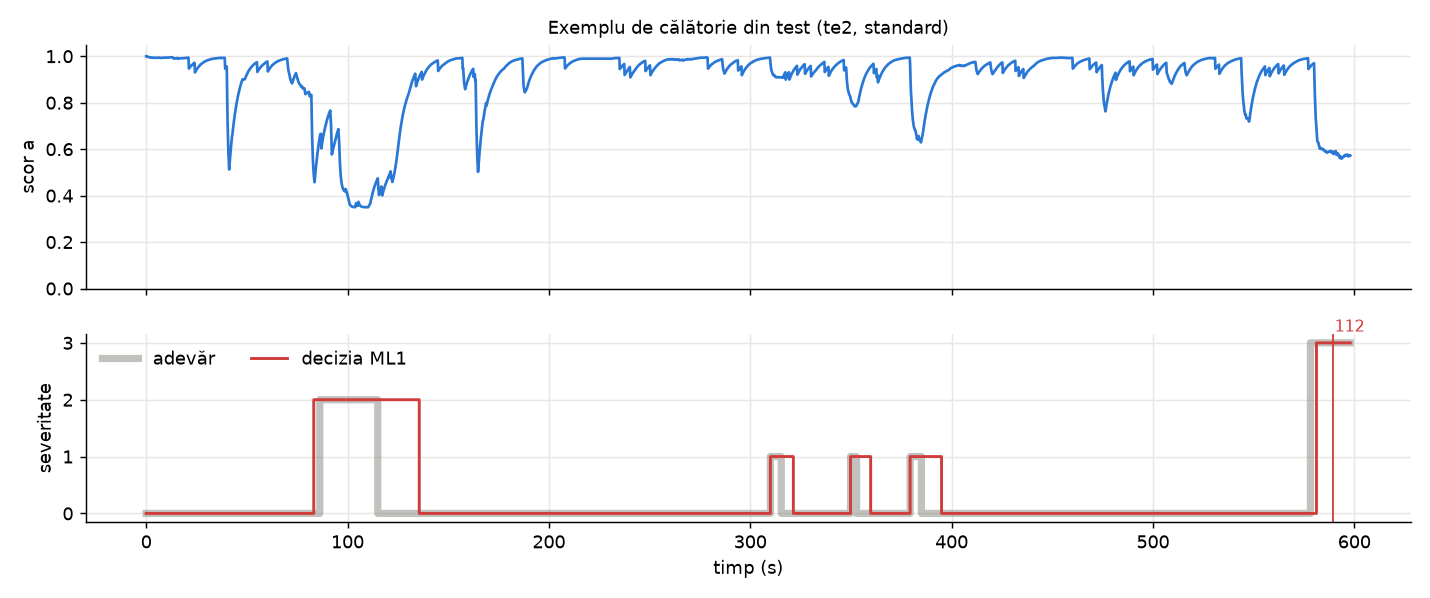
\includegraphics[width=\textwidth]{../figures/trip_example.png}\\[2pt]
{\small\color{ink2} One test trip: attention score (top); true severity (gray) vs ML1's decision (red), with the 112 call.}
\end{center}

\begin{center}
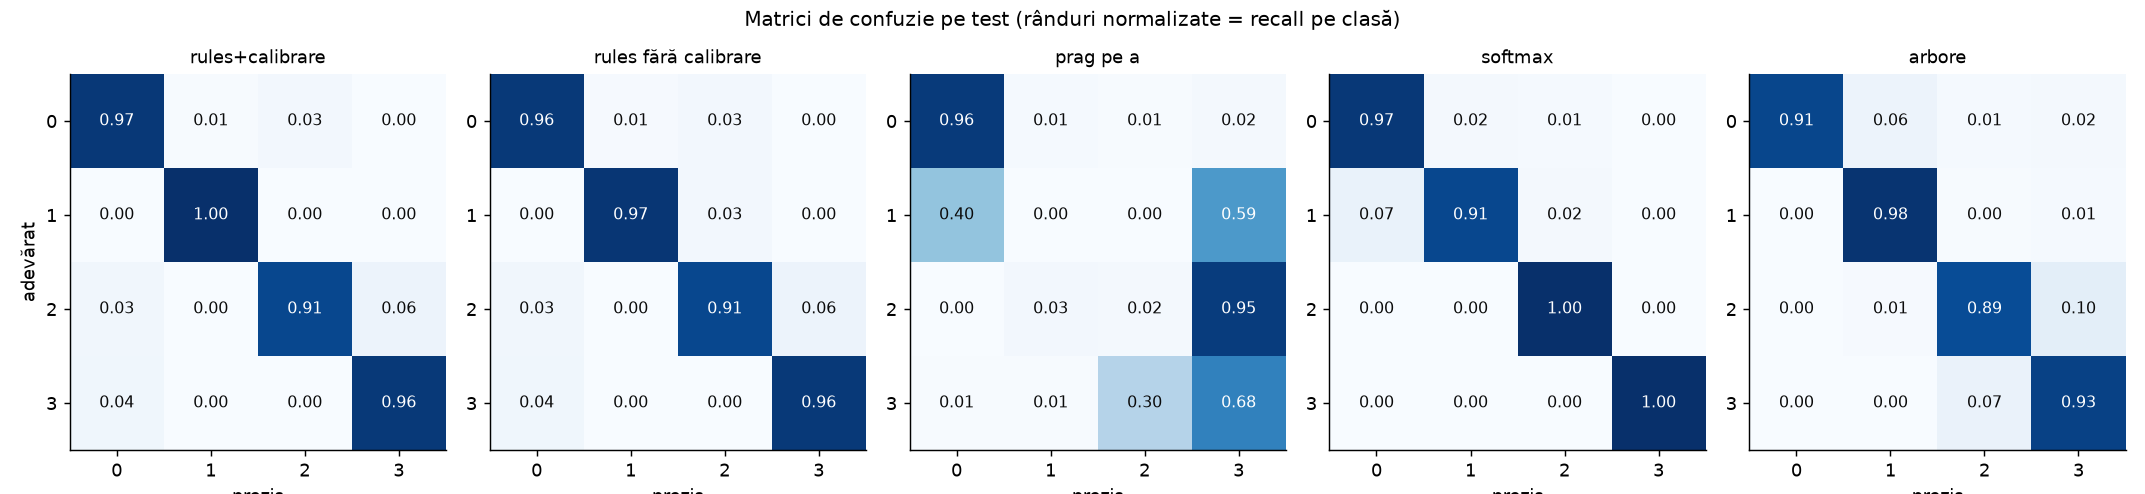
\includegraphics[width=\textwidth]{../figures/confusion_test.png}\\[2pt]
{\small\color{ink2} Confusion matrices on test, rows normalized (recall per class). The 2 $\to$ 3 cell is a tired driver who stays silent and gets escalated, by design.}
\end{center}

% ======================================================================
\section{Numbers cheat sheet}
\begin{tabularx}{\textwidth}{@{}Y l l@{}}
\toprule
\thead{Quantity} & \thead{Value} & \thead{Source} \\
\midrule
frame rate in ML1 tests / CV publish rate & 5\,Hz / 10\,Hz & simulator / CV config \\
CV event minimum durations & chest 2\,s, breathing 3\,s, phone 1\,s, wheel 2\,s & \fname{Vision/config.yaml} \\
ML1 chest threshold & 3\,s & rules \\
LLM latency & median $\approx$260\,ms, p95 $\approx$370\,ms & measured \\
prompt phase / output & 9--18\,ms / 25--42 tokens & measured \\
prompt size & 976 tokens & measured \\
model memory & 1.1\,GB, 100\% GPU, context 2048 & \code{ollama ps} \\
LLM timeout before rules take over & 2.5\,s & validate \\
detection latency (simulated) & collapse 0.2--2\,s, chest 3\,s & evaluation \\
112 after onset (simulated) & 8--11\,s & evaluation \\
test: legacy / CV-aligned / + LLM & macro-F1 0.75 / 0.83 / 0.89 & evaluation \\
shift domain without / with calibration & macro-F1 0.58 / 0.82; 62 / 20 false alarms per hour & evaluation \\
\bottomrule
\end{tabularx}

% ======================================================================
\section{Known limitations and open questions}
{\raggedright
\begin{enumerate}
  \item \textbf{All evaluation data is simulated.} Good for regressions and comparisons, not for real-world accuracy.
  \item \textbf{\code{confidence} is a coverage heuristic, not a calibrated probability.} ``0.6'' means ``camera only'', not ``60\% likely correct''.
  \item \textbf{Fusion weights, caps and time constants are hand-chosen.} Only \code{FACE_MISSING_SEC},
        \code{LOW_A_PERSIST_SEC}, \code{LLM_MAX_RAISE} and the $a$ cut points were chosen from data.
  \item \textbf{\code{answer_status} uses keyword regexes.} „Nu, sunt bine” (``No, I'm fine'') is read correctly;
        „nu știu” (``I don't know'') becomes ``slow''. Real speech-recognition output will be messier.
  \item \textbf{The LLM's gain over the rules has overlapping confidence intervals}, and \code{LLM_MAX_RAISE} was
        chosen after a test result had been seen, so the test number is slightly optimistic.
  \item \textbf{Severity-2 recall is about 0.79}: a tired driver who stays silent gets escalated to 3 (intended, but it costs severity-3 precision).
  \item \textbf{The MQTT bridge is untested against a real broker} and needs \code{paho-mqtt}.
  \item \textbf{One trip state.} The engine assumes one driver per process; a driver change mid-trip would need recalibration.
  \item \textbf{Prefix caching is inferred from timings}, not from server internals; another inference server may behave differently.
\end{enumerate}
\par}

% ======================================================================
\section{Hands-on exercises}
Run from the repository root. Each exercise builds one intuition.

\begin{trybox}[1 · Trace a frame yourself]
\begin{codeblock}
python -c "from ml1.cv_adapter import cv_demo_messages as m; from ml1.engine import DecisionEngine as E; e=E(); [e.on_vision(x) for x in m() if x['ts']<=45]; print(e.last_result.to_dict())"
\end{codeblock}
Recompute $a_\text{raw}$ by hand from the contributions and the events cap. You should get 0.568.
\end{trybox}

\begin{trybox}[2 · Watch smoothing]
\code{python -m ml1.replay tests/data/glance.jsonl --every 1}: a 1\,s glance barely moves $a$. Set
\code{TAU_DOWN = 0.1} in \fname{fusion.py} and replay. What would the driver hear?
\end{trybox}

\begin{trybox}[3 · Break the ladder order]
In \fname{rules.py}, move the ``eyes closed $\ge$ 1.5\,s $\to$ 2'' rung above ``eyes closed + no answer $\to$ 3'' and run
\code{python -m unittest tests.test_integration_cv}. Which test catches it?
\end{trybox}

\begin{trybox}[4 · See the guards work]
\begin{codeblock}
python -m unittest tests.test_validate -v
\end{codeblock}
Each of the 26 cases in \fname{tests/data/llm_outputs.json} is a way
an LLM can fail. Pick three and predict the outcome before reading the test.
\end{trybox}

\begin{trybox}[5 · Feel calibration]
Run \code{python -m ml1.evaluate --quick} and compare ``rules fără calibrare'' with ``rules+calibrare'' on
\code{shift}. Then set \code{PERCLOS_MAX = 0.40} in \fname{calibration.py} and rerun: what risk does that create?
\end{trybox}

\begin{trybox}[6 · Measure the LLM]
\code{python -m ml1.bench --runs 5}, then set \code{num_predict} to 16 in \fname{llm_client.py}, warm up, and rerun.
Latency drops; does validity hold?
\end{trybox}

\begin{trybox}[7 · Async race]
Read \code{test_fast_path_does_not_wait_for_slow_llm} and \code{test_stale_llm_answer_discarded} in
\fname{tests/test_engine.py}, then explain the two discard conditions of \code{_llm_job} in your own words.
\end{trybox}

\begin{trybox}[8 · Dashboard intuition]
\code{python -m ml1.dashboard --autostart cv_demo --speed 2}, then hover the score chart around the chest phase and find
the moment \code{capped_by} switches to \code{events}.
\end{trybox}

% ======================================================================
\section{Further reading}
\subsection*{Course (in this repository)}
\begin{itemize}
  \item \fname{ML_C2.pdf}: missing-data mechanisms, robust scaling, fit/transform without leakage (3.2, 3.3)
  \item \fname{ML_C4.pdf}: probability vs decision threshold, softmax, cross-entropy (3.7, Section 4)
  \item \fname{ML_C5.pdf}: splits by subject, per-class metrics, cost-based thresholds, bootstrap, calibration, distribution shift (Section 4)
  \item \fname{ML_C6.pdf}: decision trees and inductive bias (the tree baseline)
\end{itemize}
\subsection*{External}
Look these up in the original before citing; titles are given so they can be found.
\begin{itemize}
  \item Ollama documentation, ``Structured outputs'' (the \code{format} parameter), and the llama.cpp GBNF grammars README: how schema-constrained decoding works.
  \item Qwen2.5 Technical Report (arXiv 2412.15115) and the Llama 3.2 model card: capabilities and licenses.
  \item Dinges \& Grace (1998), ``PERCLOS: A valid psychophysiological measure of alertness as assessed by psychomotor vigilance'' (FHWA tech brief).
  \item Åkerstedt \& Gillberg (1990), ``Subjective and objective sleepiness in the active individual'': the Karolinska Sleepiness Scale, for labeling real drowsiness data.
  \item Regulation (EU) 2019/2144 (General Safety Regulation): the DDAW/ADDW requirements behind the pitch.
  \item ISO 26262 (functional safety) and ISO 21448 / SOTIF (safety of the intended functionality, including sensor and ML limits).
  \item Efron \& Tibshirani, \emph{An Introduction to the Bootstrap}: the confidence-interval method in Section 4.
\end{itemize}

\end{document}
